% DSD Lab3 report

\documentclass[10pt]{article}
\usepackage{mathtools, amsmath, amsfonts, amssymb}
\usepackage{hyperref, graphicx, wrapfig, geometry}
\usepackage[makeroom]{cancel}

\usepackage[section]{placeins}
\newgeometry{margin=2cm}

\title{ECSE 323 --- Group 47 Lab 3 Report}
\author{Junyoung Shin id. 260499663\\ Timothee Flichy id. 260557686}
\date{\today}

\begin{document}
\maketitle
\section*{Design and simulation of a 0-to-25 Counter Circuit}
We desiged a 0-to-25 counter with inputs clock, asynchronous reset, and count\_enable. The counter gives a 5-bit output which counts up every clock cycle while count\_enable is high and reset is high. The count\_enable and count are triggered at the rising edge of the clock. The count will add 1bit every clock cycle until it reaches the max value of $"11001"$ or 25. When reset goes low, the count goes to $"00000"$. If count\_enable is not set high, the count is will hold its value until count\_enable goes high.
To test our code, we created a clock pulse of 50ns and tested the VHDL code. The data of the test cana be seen on figure \ref{fig:count_test}.
\begin{figure}[!htb]
    \centering
    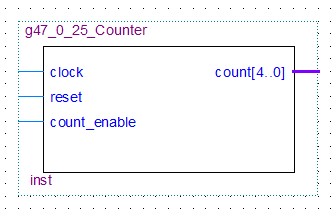
\includegraphics[width=0.5\textwidth]{./counter_0to25.png}
    \caption{0-to-25 counter pin-diagram.}
    \label{fig:count_pin}
\end{figure}
\begin{figure}[!htb]
    \centering
    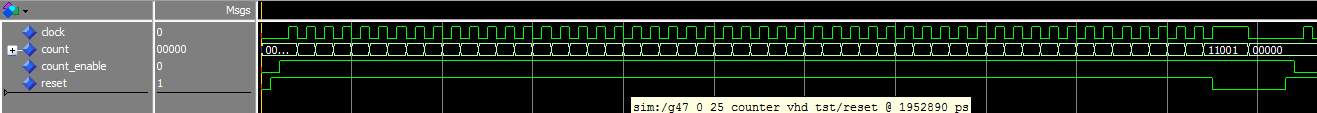
\includegraphics[width=1\textwidth]{./test_0to25.png}
    \caption{Simulation of the 0-to-25 counter.}
    \label{fig:count_test}
\end{figure}
\section*{Testing the 7-segment LED decoder on the Altera Board}
The Altera DE1 development board is equiped with 4 7-segment LED displays and 10 simple switches which are processed by the FPGA. Our goal was to  to make the LED display letters in the alphabet when toggling 5 of the switches availabe on the board. The encoding configuration is displayed in table \ref{tab:alph_label}.
\begin{table}[!htb]
    \caption{Alphabetical value accoding to the 5bit code.}
    \label{tab:alph_label}
    \centering
    \begin{tabular}{l|cc}
    \hline
    \hline
    \textbf{Code} & \textbf{Letter}\\
    \hline
        \verb@00000@ & A \\
        \verb@00001@ & B \\
        \verb@00010@ & C \\
        \verb@00011@ & D \\
        \verb@00100@ & E \\
        \verb@00101@ & F \\
        \verb@00110@ & G \\
        \verb@00111@ & H\\
        \verb@01000@ & I\\
        \verb@01001@ & J\\
        \verb@01010@ & K\\
        \verb@01011@ & L\\
        \verb@01100@ & M\\
        \verb@01101@ & N\\
        \verb@01110@ & O\\
        \verb@01111@ & P\\
        \verb@10000@ & Q\\
        \verb@10001@ & R\\
        \verb@10010@ & S\\
        \verb@10011@ & T\\
        \verb@10100@ & U\\
        \verb@10101@ & V\\
        \verb@10110@ & W\\
        \verb@10111@ & X\\
        \verb@11000@ & Y\\
        \verb@11001@ & Z\\
    \hline
    \hline
    \end{tabular}
\end{table}
To decode the binary numbers being put in by the swtiches, we used the 7\_segment\_decoder to show the letters according to the table \ref{tab:alph_label}.
The second step was to make a testbed circuit which combined all the components we have made so far including: 26\_5\_encoder, 5\_26\_decoder, 0\_25\_counter, pulse\_generator, 26\_barrelshift, and 7\_segment\_decoder. The testbed also used 5 switches to set the inital shift amount then shifts up using the 26\_barrelshift circuit. A pulse generator is used to create a 2Hz pulse that acts as a 0\_25\_counter enable signal. This is due to the FPGA's clock being 50MHz which is too quick for human perception. The calculation the number times the value is loaded into the circuit, we used the equation $\text{pulse}=(N+1)Tc$ where pulse if $0.5$s and $Tc=0.001s$. By substituing the numbers in, we got an $N=499$. For the rest of the circuit, there is also a reset button used to reset the counter. The counter acts as our barrelshift input.\\
To test if our pulse generator worked, we our division ratio to 1000 and ran it for 10us. By doing so, we expected to have 5 pulse in the 100us which was the case as shown in figure \ref{fig:test_bed}. To make the test work, in our pulse\_generator circuit, we changed LPM\_WIDTH=10, LPM\_MODULUS=1000, and the q to std\_logic\_vector(9 downto 0).
\begin{figure}[!htb]
    \centering
    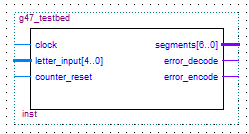
\includegraphics[width=.6\textwidth]{./segment.png}
    \caption{7 segmented display output circuit.}
    \label{fig:segment}
\end{figure}
\begin{figure}[!htb]
    \centering
    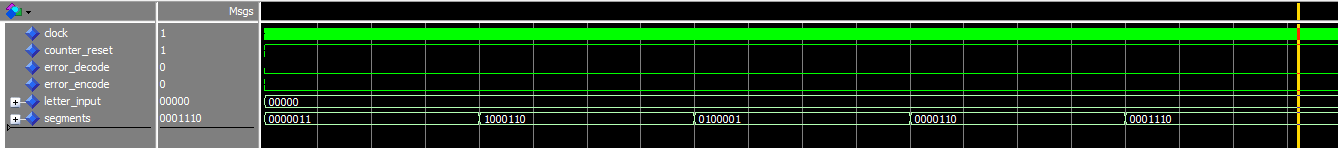
\includegraphics[width=0.8\textwidth]{./test_bed.png}
    \caption{Testing the pulse generator.}
    \label{fig:test_bed}
\end{figure}\\

For our circuit, using the Altera EP2C20F484C7N fast model hold (FMH) slack time is 0.357ns, slow model setup (SMS) slack value is 14.167ns, and the slow model Fmax (SMFm) is 185.77MHz. If we changed to the cheaper Altera 5CSEMA5F31C6 having a FMH slack time of 0.259, a SMS slack value of 13.923, and a SMFm of 164.55MHz, we can see that the chaper model still has its SMFm higher then 50MHz clock cycle. Meaning changing to the Altera 5CSEMA5F31C6 would save to company buying 100,000 units a total of 1.557 million dollars.


\end{document}